\documentclass[twocolumn]{article}
\usepackage{xurl}
\usepackage{graphicx}
\title{Medical Imaging Computing Assignment 1}

\author{Suneet Tipirneni}

\begin{document}
\maketitle
\section{Code}
Code for the assignment can be found at \url{https://github.com/suneettipirneni/med-proj-1}
\section{Task 1} \label{sec:model1}
\subsection{Training resnet-18 from scratch}

\subsubsection{Implementation}

	The model I used for this assignment was the low-fidelity resnet-18 model. For input transforms each image needed to be resized to 224 as this is what the resnet model expects as an input dimension. \par

	For the number of epochs I chose 30 as it seem to give the best balance between both computational runtime and overall accuracy. For a batch size a size of 5 was chosen as this was a similiar batch size used by \cite{transferlearning} for their model training, mine is increased by one as it helps improve how fast the model trains. The results are shown in figure \ref{fig:res1}. 


\subsubsection{Graphs}

\begin{figure}[!htb]
	\centering
	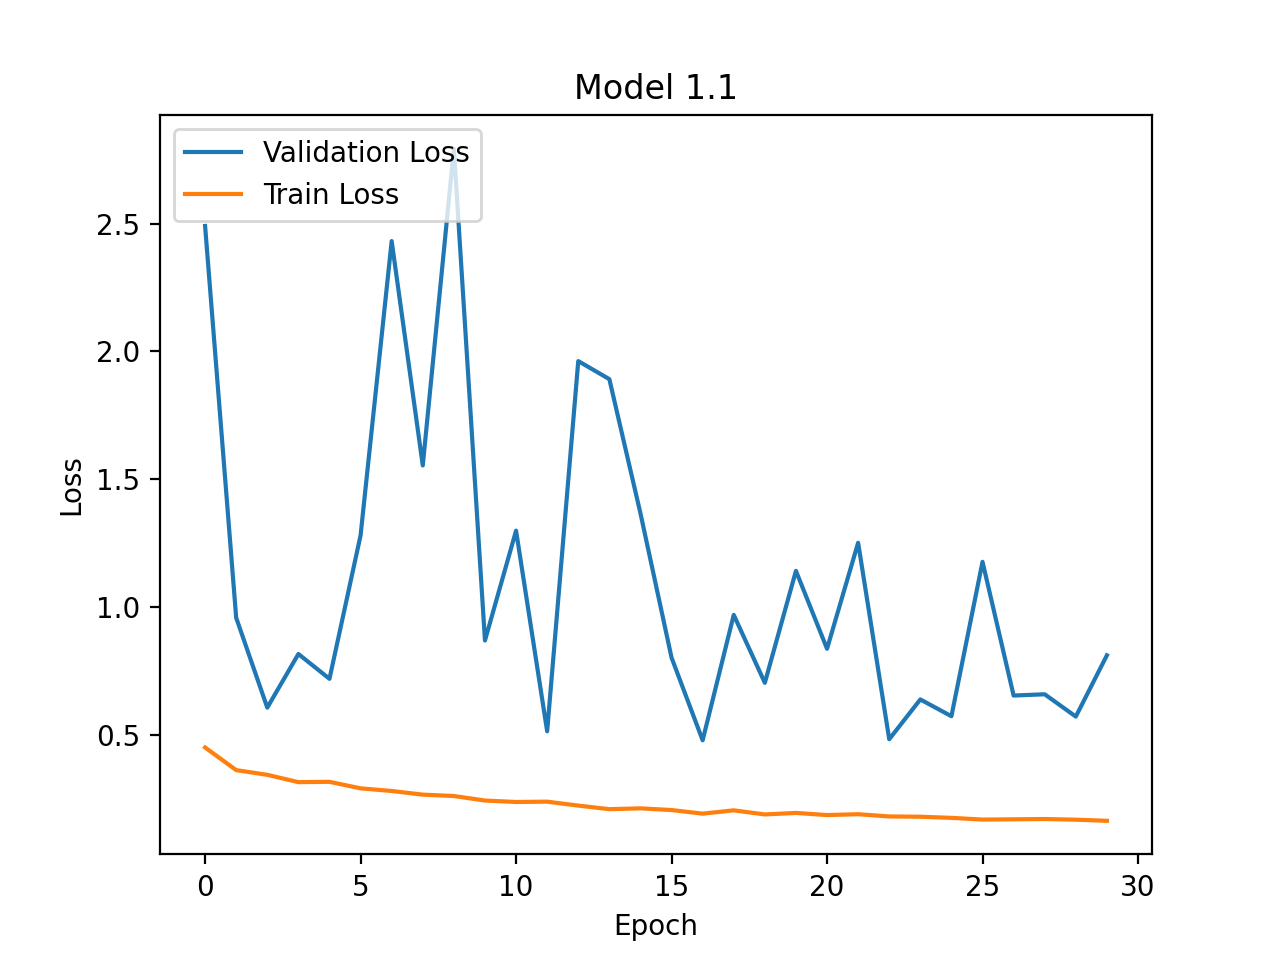
\includegraphics[scale=0.45]{model-1.1.png}
	\caption{Results from pretraining the model fully}
	\label{fig:res1}
\end{figure}

\subsubsection{Accurracies}

The overall accuracy of this model was 92\%, the outline of the different percentages for each class is shown below in table \ref{tab:1} 

\begin{table}[h]
	\begin{tabular}{ll}
		Normal    & 87\% \\
		Pneumonia & 97.4\%
	\end{tabular}
	\caption{Individual Accurracies for model 1.1}
	\label{tab:1}
\end{table}


The calculation of these individual accuracies uses the code from \cite{training}. 

\subsection{Finetuning a resnet-18}
\subsubsection{Implementation}
	For the second task a resnet-18 model was once again used, however the model was trained with it's preexisting weights that were previously learned on the ImageNet dataset.\par 

	As with the previous model, a batch size of 5 and and the number of epochs were set to 30. These values were kept the same in order to make sure a fair comparison could be formed between both models. \par

	This model mainly differs in the architecture described in section \ref{sec:model1}. A dropout layer with a rate of 0.5 is employed before the final fully-connected layer to prevent over-fitting. In addition to architecture changes, data augmentation is performed to increase the fidelity of the test dataset. Firstly, a random horizontal transformation is applied to input images, horizontal transforms were only used as opposed to vertical transformsas the body would be misrepresented by a vertical flip. Secondly, a random crop to the network input size of 224 is employed this allows the inputs to crop to a variety of different areas and helps the model to not over-train onspecific formats and shapes of images.

\subsubsection{Graphs}

\begin{figure}[!htb]
	\centering
	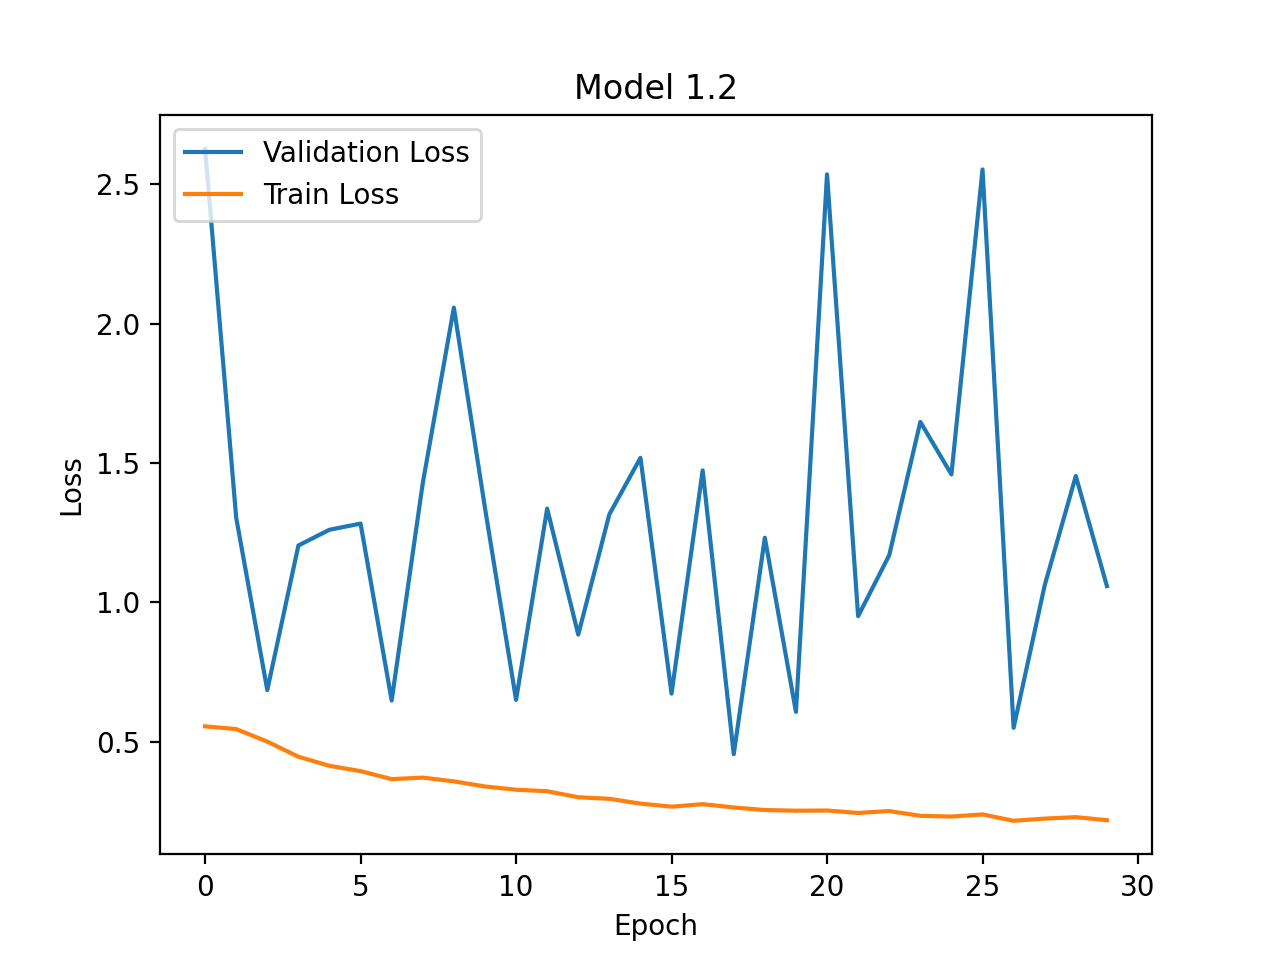
\includegraphics[scale=0.45]{model-1.2.png}
	\caption{Results from finetuning the model using pretrained resnet-18 weights}
	\label{fig:res2}
\end{figure}

\subsubsection{Accurracies}

The overall test accuracy for this model was 89\%. This was slightly lower than the previous model, this may be due to lack of training time. The per-class accuracies for this model are shown in table \ref{tab:2}.

\begin{table}[h]
    \begin{tabular}{ll}
        Normal    & 76.5\% \\
        Pneumonia & 95.4\%
    \end{tabular}
    \caption{Individual Accurracies for model 1.2}
    \label{tab:2}
\end{table}

Compared to the first model these are slightly lower scores. I once again believe this may be be caused by the lack of training time for the model. Perhaps increasing the epoch count would yield better results.

\bibliographystyle{acm}
\bibliography{references}

	
\end{document}
